% Compile with Texifier Unicode / XeLaTeX / Tectonic.
% !TEX encoding = UTF-8 Unicode
\documentclass[10pt,a4paper]{article}
\usepackage{raylo-report}
\begin{document}
\hypersetup{pageanchor=false}
\begin{titlepage}
\pagecolor{Blue}\color{white}

\includegraphics[width=30mm]{assets/raylo-white.png}\hfill {\small SEPTEMBER 2026}\par
\vspace*{27mm}
{\small\bfseries AI ACCELERATION\quad /\quad RESEARCH REPORT\par}
\vspace{10mm}
{\fontsize{36}{40}\selectfont\bfseries Open Banking\\Transaction\\Categorisation\\and Credit Risk\par}
\vspace{12mm}
{\large A taxonomy Raylo owns, the pipeline that applies it, the models tested for the hardest part of that pipeline, and the evidence that the resulting features improve credit decisions.\par}
\vfill
\vspace{10mm}
{\small Carlos Noble Jesus | AI Engineering\hfill Updated 7th September 2026}
\vspace{5mm}
%{\footnotesize Confidential, internal use only\hfill raylo.com\par}
\end{titlepage}
\hypersetup{pageanchor=true}
\nopagecolor\color{Charcoal}
\section*{Abstract}
Raylo's live Open Banking risk model reads Plaid's category names directly, which leaves a core model input outside our control. This report describes the taxonomy built to replace that dependency (275 detailed categories rolling up to 29 general ones), the seven-tier pipeline that applies it, and the modelling work completed since the August report.

On 2,000 held-out transactions the full pipeline now assigns the correct detailed category 83\% of the time. The provider's own category, which is what the live model consumes, is right 30\% of the time on the same rows. For the machine-learning tier that handles the transactions rules cannot, a transformer pretrained on 21.5 million bank narratives and taught from 405,000 consensus-labelled texts beats the linear classifier by five points on never-seen merchants and by ten points on high-risk categories, with confidence intervals that exclude zero.

On the credit side, a champion model built on leaf-level taxonomy features reaches a GINI of 0.62 on the six-month arrears outcome against 0.42 for the live model, up from the 0.56 quoted in August. Most of that gain comes from the model seeing thousands of leaf-level columns. Held to a governable 50 features and a single XGBoost, the same recipe scores 0.59, and that capped model is the one carried forward. A separate programme tested whether a sequence transformer reading raw transactions could beat it; on its own it could not. Added to the 50-feature model as single columns, however, a text-encoder score and a sequence-encoder score each give a clear lift, and together take the model to 0.63, above the uncapped champion. The text-score recipe is locked; the two-score version is the registered challenger for the prospective test.


\clearpage
\tableofcontents

\clearpage
% Edit this section directly. Styling is in raylo-report.sty.
\section{Why a taxonomy Raylo owns}
Raylo's live Open Banking risk model is an XGBoost trained on features derived from Plaid's category names. That is fragile in two ways.

First, we do not control the definitions. Plaid shipped a new taxonomy version in December 2025, months after Raylo went live on Plaid in August 2025. The same transaction can be relabelled between versions, which silently changes what the model's features mean without anything failing a test.

Second, providers disagree with each other. We hold two sources: Equifax (through its AccountScore engine), a closed one-time dump of 73 million transactions covering July 2022 to September 2025, and Plaid, live since August 2025 with 4.3 million transactions and growing. For the roughly 2,300 merchants both providers cover, their categorisations give different answers for 72\% of merchants and 45\% of volume. Uber Eats is a takeaway in one and a restaurant in the other. Marks and Spencer is a credit-card repayment in Equifax, because Equifax matched M\&S Bank, and a department store in Plaid. A crosswalk that simply maps one scheme onto the other carries every one of those conflicts through, and any model trained on Equifax history and served on Plaid traffic inherits them.

The aim is therefore a taxonomy that Raylo defines and governs, where the providers' categories are treated as one piece of evidence rather than as the definition. Everything else in this report follows from that decision.


% Edit this section directly. Styling is in raylo-report.sty.
\section{Designing the taxonomy}
The taxonomy has two levels: 275 detailed categories, which we call leaves, rolling up into 29 general categories. It was verified programmatically to leave no uncovered value across all 255 Equifax subcategories, 47 Equifax primary categories and 91 Plaid detailed categories, so any transaction either provider can describe has a home.

Three design decisions shaped it.

\subsection{Cross-cutting concerns are flags, not levels of the hierarchy}
Whether a category is essential spending, whether it is debt, whether it is a priority debt in the UK debt-advice sense, whether it is age-restricted, and whether it carries a risk flag are all recorded as separate attributes of each leaf. They cannot be levels in a tree because they are not tree-shaped: rent and mortgage are both essential, but only mortgage is debt. Folding debt into the hierarchy would have made an essential-spend feature exclude mortgage for homeowners and include rent for renters, a tenure-based distortion inside a credit decision with obvious fairness implications.

\subsection{Predictive power does not decide which categories exist}
An early version pruned leaves that did not predict arrears and had to be rebuilt. Low predictive power only tells you where it is safe to aggregate for one particular outcome. The clearest case is gambling: the combined gambling category carries almost no signal, while lottery alone carries the strongest signal of any gambling subtype. Merging the subtypes would have destroyed information that later turned out to matter, and a test now guards against it.

\subsection{The general level is a strict rollup}
Every leaf has exactly one parent. Equifax's own two category fields are not a hierarchy (222 of its 255 subcategories appear under multiple primaries), which is part of why its output is hard to reason about. A strict tree means a general-level feature always means the same thing.


% Edit this section directly. Styling is in raylo-report.sty.
\section{How many categories is the right number}
Stakeholders asked whether 275 was too many, too few, or arbitrary. We tested both directions, and the answer turned out to depend on the model that consumes the categories, so it is given in two parts.

Collapsing, with the simple August model: the same features were rebuilt at seven levels of detail from 275 leaves down to 4 broad groups, and the August XGBoost trained at each, three seeds with bootstrap intervals. The 275-leaf, 69-group and 29-group views were statistically indistinguishable. Seventeen groups was close but showed a small, real loss on the six-month outcome. Nine and fewer degraded clearly. The 69-group view is worth explaining because it causes confusion: it is today's model-feature grouping, in which 40 leaves each get their own feature block and the other 235 are rolled into their 29 general categories. All 275 leaves are still classified; none are dropped.

Collapsing, with the champion recipe of section 10: the same ladder was re-run with the stronger recipe and its richer per-category features once that became the reference model. Given every column, the six-month outcome now rewards detail: 275 leaves scores 0.612 against 0.586 for today's 69 groups, falling steadily to 0.510 at 4 groups. The three-month outcome does not; its peak is the 69-group view and 275 sits marginally below it. Under a hard 50-feature cap the picture inverts. The 275-leaf rung becomes the worst on both outcomes, because roughly 2,900 thin per-leaf candidates crowd the handful of broad, information-dense features (priority-debt breadth, months with credit products) out of the 50 slots: only 2 of those 31 spine columns survive selection at 275 leaves, against 9 at 17 groups. That is a property of feature selection from a very wide pool, not of the taxonomy, and it is why the capped champion in section 10 selects from a base that keeps those spine features rather than from the raw leaf pool.

Expanding: three well-supported parents (streaming, general marketplace, payment intermediary) were split into 15 shadow children, a simulated move from 275 to 287 leaves, with the rules frozen before any outcome was inspected. Against a control that received the exact parent totals, the split features changed GINI by between minus 0.002 and minus 0.011, with every confidence interval including zero. Payment intermediary on its own produced a small but clear loss. This was not a thin-data result: the shadow categories appeared in 54,000 of 64,000 modelling rows.

\begin{figure}[H]
\centering
\ChartTitle{Figure 1. Risk-model GINI by number of category groups, August recipe (same cohort, same learner, 3 seeds)}
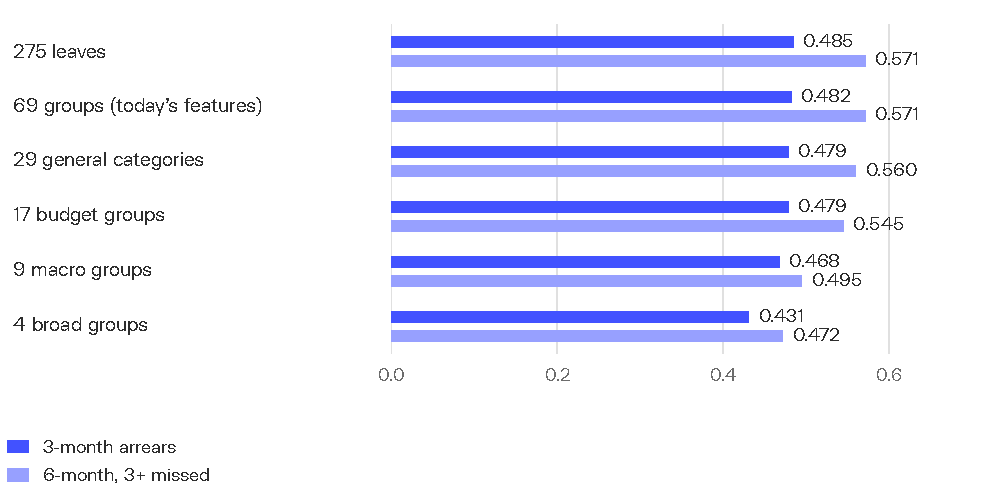
\includegraphics[width=\linewidth]{charts/fig-ladder.pdf}
\caption*{August recipe: a single XGBoost on rung-level counts and amounts, uncapped, 3 seeds. Collapsing the 275 leaves to 69 or 29 groups costs nothing measurable; 17 begins to lose the six-month signal; 9 and fewer degrade clearly. Predates the September as-of rebuild; directional.}
\end{figure}
\begin{figure}[H]
\centering
\ChartTitle{Figure 2. The same ladder with the champion recipe, six-month GINI, single XGBoost}
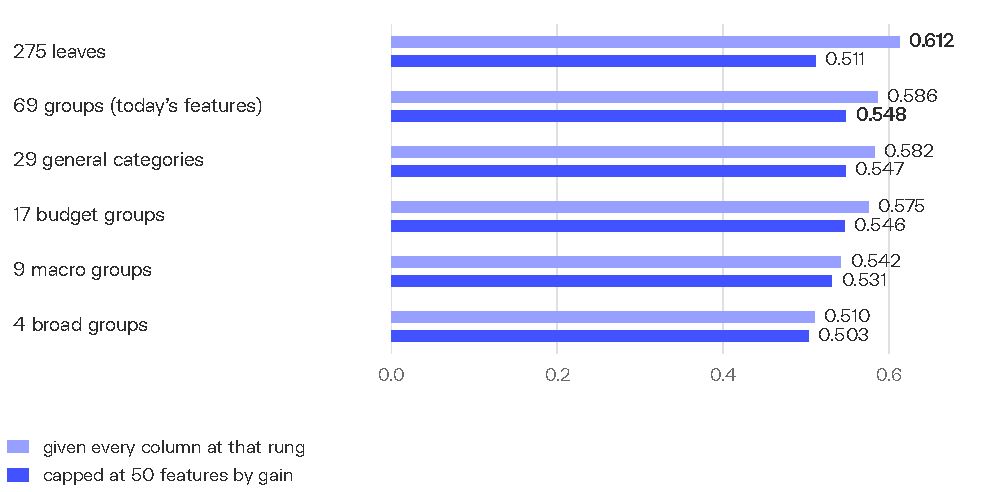
\includegraphics[width=\linewidth]{charts/fig-ladder-champ.pdf}
\caption*{Champion recipe with its richer per-category features, rebuilt at each rung on a recipe-neutral base so only granularity changes. Given every column, finer is better on the six-month outcome. Capped at 50, the 275-leaf rung is worst because its 2,900 thin candidates crowd the strongest broad features out of the selection. The three-month outcome shows no gain from detail in either setting; 69 groups is its peak.}
\end{figure}
\subsection{Reconciling the two results}
The two ladders look contradictory and are not. They answer different questions, and the same three facts hold across both.

\begin{enumerate}
\item \textbf{Whether detail helps depends on what the model can do with it.} The August model built one count and one amount per category. At that level of description, 275 leaves carried no more usable signal than 29 groups, because most of what a leaf adds over its parent is in how the spending is distributed, not in its total. The champion builds per-leaf shares and averages, and with those in hand the six-month model finds real signal in the fine leaves. The three-month horizon is noisier and shorter, and does not, under either recipe.
\item \textbf{A hard feature cap is a selection problem, not a taxonomy problem.} Ranking 2,900 candidate columns by gain and keeping 50 is unreliable: thin per-leaf columns outnumber the handful of broad, strong features by a hundred to one, and the strong ones are squeezed out. That is why the 275-leaf rung scores worst when capped from the raw pool. The capped champion in section 10 avoids this by selecting from a base that already contains the broad features alongside the leaf-level ones, and reaches 0.588 where the raw-pool rung reaches 0.511.
\item \textbf{The taxonomy decision is the same under every reading.} Categories are stored at 275 leaves because a leaf can always be rolled up at feature-build time and a rollup can never be split back. Which rollup or feature pool a given model consumes is a modelling choice, made per model and per outcome, and validated the way the capped champion was.
\end{enumerate}
\begin{tcolorbox}[colback=BlueTint,colframe=Blue,boxrule=0pt,leftrule=2pt,arc=3mm]
Keep 275 leaves as the governed source of truth. Detail is reversible, since a leaf can be rolled up at feature-build time, while deletion is not, and the stronger the model, the more the six-month outcome rewards that detail. Let each model consume a validated rollup or a curated feature pool, and keep proposed new categories in shadow until they show stable value.
\end{tcolorbox}

% Edit this section directly. Styling is in raylo-report.sty.
\section{Labelling the data}
A taxonomy is only useful with labelled examples behind it, and the labelling has to be trustworthy enough to serve as ground truth. The approach settled on has four parts.

\subsection{Two models must agree}
Before committing to a large build, a cheap gating experiment had two large language models independently label the 2,300 merchants both providers cover. Raw agreement with Equifax's labels looked poor, but the benchmark itself was the problem: Equifax's "truth" is its own dictionary conventions, some of which our taxonomy rejects on purpose (Equifax files Netflix under broadband and Boots under beauty). Human review of the disputes gave a corrected accuracy of 96\% at leaf level, and set two standing rules. Two models must agree, with the option to abstain rather than guess. And no language model ever runs at decision time; they label offline, and small fast models are trained from those labels.

The production committee is Gemini Flash and Claude Sonnet, chosen from a six-model benchmark, with Claude Opus as a tiebreak where a human will review the result. When we later measured the committee's output against Carlos's own labels on the credit tranche, rows where the two models agreed were 95\% correct at leaf level. Rows accepted through the tiebreak were only 64\% correct, so tiebreaks are now used only for tranches that go to human review, never for training data.

\subsection{Targeted human review}
Human review is spent where it pays most: on disputes between the models, on high-risk categories, and on blind slices that measure the committee's accuracy. The conventions that come out of that review (Creditspring is not payday lending, an in-store cash machine is a cash withdrawal, a bookmaker credit is winnings) are written down and applied to every later tranche.

\subsection{What was labelled}

{\small
\setlength{\TableWidth}{\dimexpr\linewidth-6\tabcolsep\relax}
\begin{longtable}{>{\raggedright\arraybackslash}p{0.29\TableWidth}>{\raggedright\arraybackslash}p{0.26\TableWidth}>{\raggedright\arraybackslash}p{0.45\TableWidth}}
\rowcolor{BlueTint}
\bfseries Dataset & \bfseries Size & \bfseries Purpose \\ \midrule
\endfirsthead
\rowcolor{BlueTint}
\bfseries Dataset & \bfseries Size & \bfseries Purpose \\ \midrule
\endhead
Merchant labels, four tranches & 100,000 merchants & Source of the merchant dictionary and of classifier training data. Provenance is tagged: human, model consensus, tiebreak. \\ \addlinespace[4pt]
Credit tranche (September) & 30,379 rows & Money-in transactions were 0.65\% of the training data and a quarter of live traffic. Carlos reviewed 813 rows; blind-slice agreement with the committee was 84\%. \\ \addlinespace[4pt]
Risk tranche (September) & 4,998 rows & Debits that look like high-risk categories (card repayments, overdraft fees, loan repayments) and that reach the ML tier. \\ \addlinespace[4pt]
Distillation labels (September) & 404,982 texts & The 500,000 most frequent distinct Plaid texts, labelled by both models; the 81\% where they agreed are kept as training signal for the transformer. Never served, never used as an evaluation set. \\ \addlinespace[4pt]
\bottomrule
\end{longtable}}
\subsection{How performance is measured}

{\small
\setlength{\TableWidth}{\dimexpr\linewidth-6\tabcolsep\relax}
\begin{longtable}{>{\raggedright\arraybackslash}p{0.29\TableWidth}>{\raggedright\arraybackslash}p{0.26\TableWidth}>{\raggedright\arraybackslash}p{0.45\TableWidth}}
\rowcolor{BlueTint}
\bfseries Evaluation set & \bfseries Rows & \bfseries Question it answers \\ \midrule
\endfirsthead
\rowcolor{BlueTint}
\bfseries Evaluation set & \bfseries Rows & \bfseries Question it answers \\ \midrule
\endhead
Merchant-disjoint holdout & 1,055 & How does the classifier cope with a merchant it has never seen? Every merchant here is excluded from all training data. \\ \addlinespace[4pt]
Risk-category gold set & 711 & Can it be trusted on gambling, debt repayment and high-cost credit? Stratified at about 20 rows per category, because volume-weighted samples starve exactly these categories. \\ \addlinespace[4pt]
Full-pipeline evaluation set & 2,000 & What accuracy does a real transaction experience end to end? Disjoint by row from training. \\ \addlinespace[4pt]
Credit evaluation set & 2,000 & Accuracy on money-in transactions specifically, merchant-disjoint. \\ \addlinespace[4pt]
Risk debits reaching the ML tier & 400 & The honest risk number: rows that look like risk categories and that the rules do not catch. \\ \addlinespace[4pt]
Locked confirmation set (v6) & 1,100 & Never scored during development. Used once, at go/no-go, so its verdict stays unbiased. \\ \addlinespace[4pt]
\bottomrule
\end{longtable}}

\clearpage
% Edit this section directly. Styling is in raylo-report.sty.
\section{The categorisation pipeline}
Every transaction resolves at the first tier that fires, and records which tier decided it. Provenance is mandatory. "Resolved by exact merchant match on Tesco" is defensible in a fair-lending review; "the model predicted 0.87" is much weaker. The deterministic tiers run first, the machine-learning tier serves what they miss, and the provider's own category is used only when nothing else can decide.

\begin{tcolorbox}[colback=BlueTint,colframe=BlueTint,arc=2mm]
\textcolor{Blue}{\textbf{T1}}\quad \textbf{Direction-dependent overrides.} A bookmaker credit is winnings, not a stake. A supermarket credit is a refund, not a shop.
\end{tcolorbox}
{\small\color{Muted} no match $\downarrow$\par}
\begin{tcolorbox}[colback=BlueTint,colframe=BlueTint,arc=2mm]
\textcolor{Blue}{\textbf{T2}}\quad \textbf{Compound merchant-plus-narrative rules.} Plaid collapses Tesco Bank, Tesco Petrol and Tesco Phone Insurance onto bare "Tesco"; narrative checks split them before the dictionary can say "groceries". HMRC child benefit credits versus tax payments are the same shape.
\end{tcolorbox}
{\small\color{Muted} no match $\downarrow$\par}
\begin{tcolorbox}[colback=BlueTint,colframe=BlueTint,arc=2mm]
\textcolor{Blue}{\textbf{T3}}\quad \textbf{Mechanism overrides.} Equifax's "Identified Salary" is salary regardless of merchant, even salary paid by a supermarket. Thirteen such primaries decide the category on their own.
\end{tcolorbox}
{\small\color{Muted} no match $\downarrow$\par}
\begin{tcolorbox}[colback=BlueTint,colframe=BlueTint,arc=2mm]
\textcolor{Blue}{\textbf{T4}}\quad \textbf{Merchant dictionary, 90,264 curated entries.} Overrides both providers on any exact match. This is the tier that makes the taxonomy provider-independent.
\end{tcolorbox}
{\small\color{Muted} no match $\downarrow$\par}
\begin{tcolorbox}[colback=BlueTint,colframe=BlueTint,arc=2mm]
\textcolor{Blue}{\textbf{T5}}\quad \textbf{Deterministic regex rules, 51 of them.} Council tax, sheriff court, StepChange, card-issuer and overdraft narratives, including on blank or truncated merchants.
\end{tcolorbox}
{\small\color{Muted} no match $\downarrow$\par}
\begin{tcolorbox}[colback=BlueTint,colframe=BlueTint,arc=2mm]
\textcolor{Blue}{\textbf{T5b}}\quad \textbf{Machine-learning classifier.} Serves everything the rules miss, on CPU, with no external calls. Abstains rather than guessing when its margin is thin. The subject of sections 8 and 9.
\end{tcolorbox}
{\small\color{Muted} abstains $\downarrow$\par}
\begin{tcolorbox}[colback=BlueTint,colframe=BlueTint,arc=2mm]
\textcolor{Blue}{\textbf{T6}}\quad \textbf{Provider crosswalk.} Plaid's or Equifax's own category mapped onto our taxonomy, used only when the classifier abstains.
\end{tcolorbox}
{\small\color{Muted} no usable category $\downarrow$\par}
\begin{tcolorbox}[colback=BlueTint,colframe=BlueTint,arc=2mm]
\textcolor{Blue}{\textbf{T7}}\quad \textbf{Explicit unclassified.} Monitored, never guessed.
\end{tcolorbox}
On live Plaid traffic the deterministic tiers resolve about 58\% of transactions before the classifier is consulted. The dictionary alone covers 56.5\% of rows, which is 89\% of the transactions that carry a merchant name at all; 37\% arrive with the merchant field blank. Everything the rules miss goes to the classifier, and the classifier serves all of it. We tested falling back to the provider's category when the classifier was unsure, and it lowered accuracy at every threshold.

The pipeline exists in two forms that must agree: the SQL that runs in BigQuery, and a Python mirror used for evaluation. A parity check now runs the SQL's own rule bodies over the evaluation rows and asserts row-level agreement. It passes 2,000 of 2,000, and when it was first written it found that 34 hand-written rules had never fired in production because of an escaping bug in the SQL generator. That is the kind of silent failure this discipline exists to catch.


% Edit this section directly. Styling is in raylo-report.sty.
\section{Measuring honestly}
A programme review at the start of September found four measurement problems. Fixing them changed some headline numbers downward before the modelling work lifted them again, and the corrected figures are the ones used throughout this report.

\begin{itemize}
\item \textbf{The risk evaluation set had leaked into training.} Three quarters of its merchants were also in the training file through a second labelling pass. The classifier's accuracy on high-risk categories had been quoted at 86\%; measured honestly it was 63\%. Every evaluation set's merchants are now excluded from every training source, and the risk number rebuilt from that floor is reported in section 8.
\item \textbf{Money-in transactions were almost absent from training.} Credits are 25\% of live Plaid rows and 50\% of the money that moves, but were 0.65\% of the training data. The pipeline was 84\% accurate on debits and 58\% on credits. All scorers now report both directions separately.
\item \textbf{The credit-risk experiment had no as-of filter on Equifax history.} Five percent of Equifax proposals carried transactions dated after the proposal was made. Removing them did not change the headline, which confirmed the uplift was real, but it had to be checked.
\item \textbf{The Python and SQL versions of the pipeline applied tiers in a different order.} Fixed, and guarded by the parity check described above.
\end{itemize}
Two further habits apply to every comparison in sections 8 to 11. Model decisions are run with three random seeds and reported as the mean. Differences between models are given with a paired bootstrap confidence interval, and a difference counts only when that interval excludes zero.


% Edit this section directly. Styling is in raylo-report.sty.
\section{Categorisation performance against the providers}
The same 2,000 held-out transactions were scored several ways. Each step removes one of our layers: first the classifier, so the provider's category serves the residual; then the rules and dictionary entirely, so only the provider's own category remains, mapped through our crosswalk. The last of these is the status quo, since it is what the live model consumes.

\begin{tcolorbox}[colback=PeachTint,colframe=PeachTint,arc=3mm]
\begin{minipage}[t]{.30\linewidth}\raggedright{\color{Blue}\fontsize{26}{29}\selectfont \textbf{30\%}}\par\small Provider's own category alone, leaf level, all 2,000 rows\end{minipage}\hfill
\begin{minipage}[t]{.30\linewidth}\raggedright{\color{Blue}\fontsize{26}{29}\selectfont \textbf{74\%}}\par\small Our rules and dictionary, with the provider's category on what they miss\end{minipage}\hfill
\begin{minipage}[t]{.30\linewidth}\raggedright{\color{Blue}\fontsize{26}{29}\selectfont \textbf{83\%}}\par\small Our rules and dictionary, with our transformer classifier on what they miss\end{minipage}
\end{tcolorbox}
\begin{figure}[H]
\centering
\ChartTitle{Figure 3. The same 2,000 held-out transactions scored four ways}
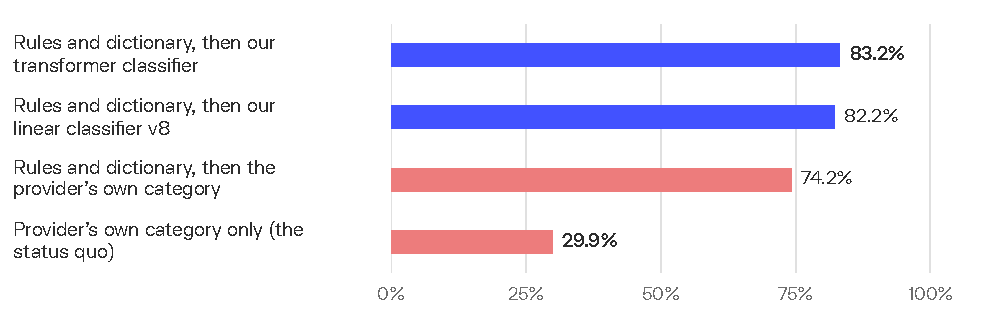
\includegraphics[width=\linewidth]{charts/fig-threeways.pdf}
\caption*{Leaf-level accuracy on the same rows. Each step down removes one of our layers. The provider's own category is what the live risk model consumes today. Rows with no provider category are counted as wrong; on provider-labelled rows alone the status quo reaches 45\%. At general level the rules-plus-classifier pipeline is 87\% and the status quo 42\%.}
\end{figure}
Where the gap comes from is worth separating. On the 1,446 rows the dictionary and early rules resolve, we are right 89\% of the time. On the Plaid rows among them where Plaid also supplies a category, we are right 92\% of the time and Plaid 32\%. Equifax is closer, at 90\% against 79\%, because its vendor field is already a curated entity and there is less for the dictionary to fix. But Equifax is a closed historical dump; live traffic is Plaid.

\begin{figure}[H]
\centering
\ChartTitle{Figure 4. Rows our dictionary and early rules resolve, where the provider also supplies a category}
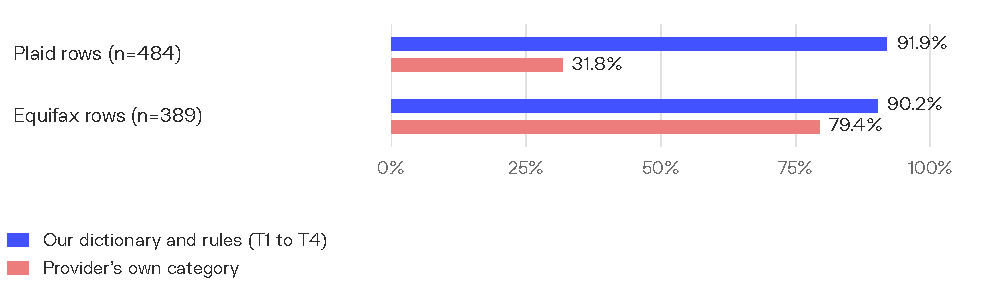
\includegraphics[width=\linewidth]{charts/fig-t14.pdf}
\caption*{Leaf-level accuracy. Plaid is where live traffic comes from and where the dictionary has most to fix; Equifax's vendor field is already a curated entity.}
\end{figure}
The residual, the 480 rows the rules cannot place, is where the machine-learning tier earns its place. There the provider's category is right 26\% of the time. Roughly half of Plaid's volume lands on coarse catch-all buckets such as "unclassified transfer", and 203 of our 275 leaves have no Plaid source at all, so categories like arranged overdraft, cash advance and pawnbroker cannot be produced from Plaid's scheme no matter how it is mapped.

\begin{figure}[H]
\centering
\ChartTitle{Figure 5. The residual: 478 rows the rules cannot place, served three ways}
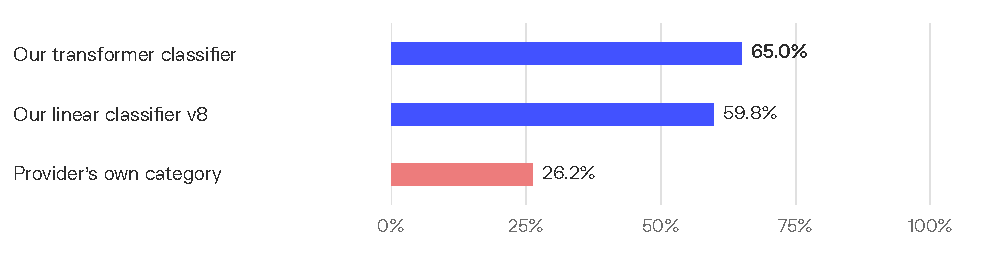
\includegraphics[width=\linewidth]{charts/fig-residual.pdf}
\caption*{This is where the machine-learning tier earns its place. Roughly half of Plaid's volume lands on catch-all buckets, and 203 of our 275 leaves have no Plaid source at all.}
\end{figure}

% Edit this section directly. Styling is in raylo-report.sty.
\section{The machine-learning tier: the linear classifier}
The classifier that has carried the residual since August is a linear support vector machine on character-level TF-IDF features. In plain terms, it counts the character fragments that appear in the merchant string and bank narrative, and learns a straight-line boundary between each category and the rest. It is the standard first model for short, noisy text: it trains in minutes, occupies 65 megabytes, scores about a thousand rows per second on one CPU core, and anything more elaborate has to beat it. It was preferred over logistic regression because it won on every promotion metric, and its ``don't answer when unsure'' behaviour works from its own decision margin.

Since August the model itself has not changed. What changed is the data it learned from, and the current version, v8, is the reference for every comparison in section 9.

\subsection{What the September data did}
The credit tranche moved accuracy on 2,000 held-out money-in transactions from 62\% to 85\%. Accuracy on debits did not move. This was the largest single-step gain in the classifier's history and it came from data, not modelling.

For high-risk categories the honest starting point, after the leak was removed, was 48\% on the 174 risk-category rows that reach the classifier. Two steps followed, in order. Five new rules for card-issuer inflows and overdraft narratives took it to 59\% before any labelling. Then 5,000 labelled rows of the same population took the classifier itself to 76\%, above the 70\% bar we set for risk categories for the first time on an honest measurement.

\begin{figure}[H]
\centering
\ChartTitle{Figure 6. Linear classifier accuracy on the two September targets, step by step}
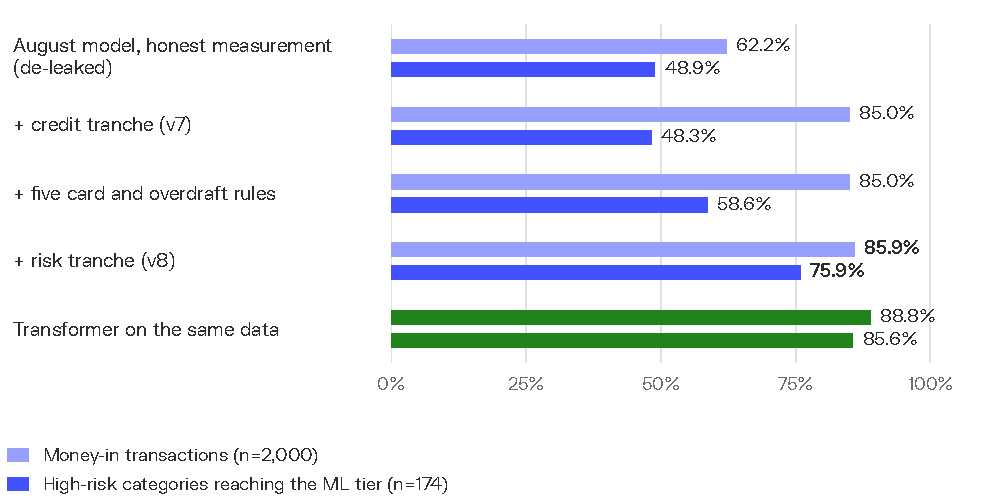
\includegraphics[width=\linewidth]{charts/fig-stair.pdf}
\caption*{The same linear model throughout; only the training data and the rules in front of it changed. The transformer row is section 9's result on identical data.}
\end{figure}
The version in the serving artefact is still v5 from August. The gap between it and v8 is now 24 points on credits and 28 points on the risk debits that reach the classifier, so promoting v8 is the zero-risk interim step whatever is decided about the transformer.


% Edit this section directly. Styling is in raylo-report.sty.
\section{The machine-learning tier: transformer models}
The linear classifier has one structural weakness. It memorises the character patterns of merchants it has seen and has no way to generalise to a merchant it has not. Frontier language models read unseen merchants at 84\% against the linear model's 54\% on the same holdout, but cannot run at decision time. The question for September was whether a small transformer, trained to run on CPU, could carry some of that reading ability into the pipeline.

\subsection{What a transformer is, in plain terms}
A transformer is a type of neural network built for sequences: words in a sentence, or here, the pieces of a bank narrative. Older text models read left to right and carried a fading memory. A transformer instead lets every piece of the input look at every other piece at once and decide how much attention to pay to each. Reading \emph{SKYBET 04321 LEEDS}, the model learns that \emph{SKYBET} is the piece that matters and that \emph{04321} and \emph{LEEDS} are a till number and a town that appear after many merchants and carry little meaning. That mechanism, called attention, is what lets the model generalise to a merchant it has never seen: it has learned which parts of a narrative tend to name the business and which are noise.

The model learns in two stages. First it is \emph{pretrained} on a very large pile of unlabelled text with a fill-in-the-blank exercise: a word is hidden and the model must guess it from the words around it. Doing this millions of times teaches it the language of the domain with no human labels at all. Then it is \emph{fine-tuned} on a much smaller set of labelled examples for the actual task, here the 275 categories. Because the pretraining already taught it what bank narratives look like, the fine-tuning needs far fewer labels than training from scratch would.

There are two families. \emph{Generative} transformers, such as the large language models used for labelling, write text out one word at a time. \emph{Encoder} transformers read text in and produce a compact numerical summary of it, a vector, which a small final layer turns into a decision. Our task is a choice from a closed list, so an encoder is the natural fit: smaller, faster, deterministic, and it cannot invent a category that does not exist.

\subsection{How our model reads a transaction}
Figure 6a follows one transaction through the model. The raw Plaid row is rewritten as a short sentence that carries everything the model is allowed to see: the direction, a coarse amount band, the merchant string and the bank narrative. That sentence is split into word-pieces, including 4,000 pieces added specifically for this domain (bank abbreviations, retailer stems, benefit codes), and each piece becomes a number. Six layers of attention then refine those numbers so that each piece is understood in the context of the others. The pieces are averaged into one 768-number summary of the transaction. Two small final layers read that summary: one scores all 275 leaves, the other all 29 general categories, and a consistency term during training keeps the two in agreement. Last, a direction mask sets to zero any category that cannot occur for that direction, so a debit can never be labelled salary. The highest remaining score is the answer, and its margin over the runner-up is the model's confidence.

\begin{figure}[H]
\centering
\ChartTitle{Figure 6a. One transaction through the categorisation transformer}
\resizebox{\linewidth}{!}{%
\begin{tikzpicture}[
  x=1mm,y=1mm,font=\footnotesize,
  box/.style={draw=Blue,fill=BlueTint,rounded corners=1.2mm,line width=0.4pt,align=center,inner sep=2.2mm,text width=30mm},
  data/.style={draw=Muted,fill=white,rounded corners=1.2mm,line width=0.4pt,align=left,inner sep=2.2mm,text width=36mm},
  result/.style={draw=Blue,fill=Blue,text=white,rounded corners=1.2mm,line width=0.4pt,align=center,inner sep=2.2mm,text width=30mm},
  lab/.style={font=\scriptsize\color{Muted},align=center},
  arr/.style={-{Stealth[length=2mm]},line width=0.5pt,color=Muted}]
  \node[data] (raw) at (0,0) {\textbf{Raw Plaid row}\\merchant: Sky Bet\\description: SKYBET 04321 LEEDS\\amount: 20.00, direction: debit};
  \node[data,text width=36mm] (sent) at (0,-24) {\textbf{One sentence}\\{\ttfamily [DEBIT] [AMT 10--50]}\\{\ttfamily sky bet | skybet 04321 leeds}};
  \node[data,text width=36mm] (tok) at (0,-46) {\textbf{Word-pieces}\\{\ttfamily debit · amt · sky · bet · sky · bet · 04321 · leeds}\\30,000 standard + 4,000 domain pieces};
  \node[box,text width=40mm,minimum height=52mm] (enc) at (62,-23) {\textbf{Encoder}\\DistilBERT, 6 layers, 66M parameters\\[3pt]Every piece attends to every other piece; \emph{skybet} is weighed up, \emph{04321} and \emph{leeds} weighed down\\[3pt]Pretrained on 21.5M transaction sentences, then taught categories from 405,000 consensus labels and the gold file};
  \node[data,text width=30mm] (vec) at (114,-23) {\textbf{One summary}\\768 numbers describing this transaction};
  \node[box,text width=30mm] (heads) at (156,-8) {\textbf{Two heads}\\275 leaf scores\\29 general scores};
  \node[box,text width=30mm] (mask) at (156,-38) {\textbf{Direction mask}\\categories impossible for a debit set to zero};
  \node[result,text width=34mm] (res) at (114,-56) {\textbf{Output}\\gambling\_betting (0.91)\\general: gambling\\margin over runner-up: 0.78};
  \draw[arr] (raw) -- (sent); \draw[arr] (sent) -- (tok);
  \draw[arr] (tok.east) -- ++(4,0) |- (enc.west);
  \draw[arr] (enc) -- (vec); \draw[arr] (vec.east) -- ++(3,0) |- (heads.west); \draw[arr] (heads) -- (mask);
  \draw[arr] (mask.south) |- (res.east);
\end{tikzpicture}}
\caption*{The sentence format gives the model what the linear classifier sees plus amount and direction. The mask is applied after the heads, so an impossible category can never win. At serving time the whole path runs on CPU at about 360 transactions a second.}
\end{figure}

What this means in practice: the linear classifier can only recognise character patterns it has already seen, so a new gambling app or a new lender is invisible to it until someone labels it. The transformer has read millions of narratives and knows what the name of a bookmaker or a lender tends to look like in a bank statement, so it gets more of them right before any label exists. That is exactly where the pipeline's remaining errors sit, which is why its gain is concentrated on never-seen merchants and on the high-risk categories.

\subsection{Why an encoder transformer, and why domain pretraining}
The output of this task is a choice from a closed list of 275 categories, which points to an encoder model with a classification head (the BERT family) rather than a generative model that writes the answer out. A fine-tuned generative model had already been tested and scored 50 to 54\% on unseen merchants, below the linear model.

Published work on transaction categorisation, including the Uncapped write-up that prompted this line of work, points to the same lesson: the gain comes from teaching the model the language of bank narratives first, not from the size of the model. Generic English encoders had already been tried here and lost; "SKY BET" and "DWP UC" are not English. So every transformer tested was first pretrained on our own transaction corpus with a fill-in-the-blank objective, with 4,000 domain-specific tokens added to its vocabulary, and only then taught the categories.

Two further design choices carried through every iteration. Each transaction is presented as a short sentence: direction, an amount bucket, the merchant and the narrative, so the model sees what the linear model sees plus amount and direction. And a direction mask at the output makes it impossible to label a debit as salary or a credit as a card payment, which removed a class of errors before training began.

\subsection{The iterations, briefly}
Eight iterations were run over four days, each against a pre-declared set of criteria and each with three seeds once a recipe stabilised. The early ones fixed bugs and established that the transformer's first apparent lead on credits was a data effect: given the same credit tranche, the linear model caught up. What did not go away was the transformer's lead on merchants it had never seen and on general-level accuracy. Three levers were then pulled in the order agreed with Carlos, each chosen because it acted on a different limitation.

\begin{enumerate}
\item \textbf{More labelled data} where the eval sets said the gap was: credits, then risk debits. Both models received it. This is section 8's story and it lifted both models equally.
\item \textbf{A larger encoder with full pretraining.} BERT-small (29 million parameters, pretrained on 3 million sentences on a laptop) was replaced by DistilBERT (66 million parameters), pretrained on the full 21.5 million-sentence corpus on a rented GPU for about seven pounds. The pre-declared rule was that under a one-point gain would close the architecture question. The result was one point on generic novel strings but four to five points on the risk set and three to four more at general level, so the larger encoder was kept.
\item \textbf{Distillation from the labelling committee.} Instead of a first training pass on labels derived from our own rules, the encoder's first pass used the 405,000 texts where Gemini and Sonnet agreed. The idea is that the committee's conventions on the common texts, which the linear model also memorises, are carried by the encoder to texts it has never seen. This added a further one to two points on every cut.
\end{enumerate}
\subsection{The result}

{\small
\setlength{\TableWidth}{\dimexpr\linewidth-10\tabcolsep\relax}
\begin{longtable}{>{\raggedright\arraybackslash}p{0.34\TableWidth}>{\raggedright\arraybackslash}p{0.1\TableWidth}>{\raggedright\arraybackslash}p{0.15\TableWidth}>{\raggedright\arraybackslash}p{0.15\TableWidth}>{\raggedright\arraybackslash}p{0.26\TableWidth}}
\rowcolor{BlueTint}
\bfseries Evaluation cut & \bfseries n & \bfseries Linear v8 & \bfseries Transformer & \bfseries Difference, 95\% CI \\ \midrule
\endfirsthead
\rowcolor{BlueTint}
\bfseries Evaluation cut & \bfseries n & \bfseries Linear v8 & \bfseries Transformer & \bfseries Difference, 95\% CI \\ \midrule
\endhead
Never-seen merchants reaching the ML tier & 416 & 59.4\% & 64.5\% & +5.1 [+1.8, +8.8] \\ \addlinespace[4pt]
Pipeline residual, the rows rules miss & 478 & 59.8\% & 65.0\% & +5.2 [+2.0, +8.2] \\ \addlinespace[4pt]
Money-in transactions & 2,000 & 85.9\% & 88.8\% & +2.9 [+1.8, +4.2] \\ \addlinespace[4pt]
\rowcolor{PeachTint}
High-risk categories reaching the ML tier & 174 & 75.9\% & 85.6\% & +9.8 [+5.2, +15.1] \\ \addlinespace[4pt]
Full pipeline, rules then model & 2,000 & 82.2\% & 83.2\% &  \\ \addlinespace[4pt]
General-level accuracy, same cuts &  &  & +7 to +13 points &  \\ \addlinespace[4pt]
Throughput, one CPU process &  & \textasciitilde{}1,050 rows/s & 360 rows/s &  \\ \addlinespace[4pt]
\bottomrule
\end{longtable}}
\begin{figure}[H]
\centering
\ChartTitle{Figure 7. Transformer minus linear classifier v8, percentage points, with 95\% confidence intervals}
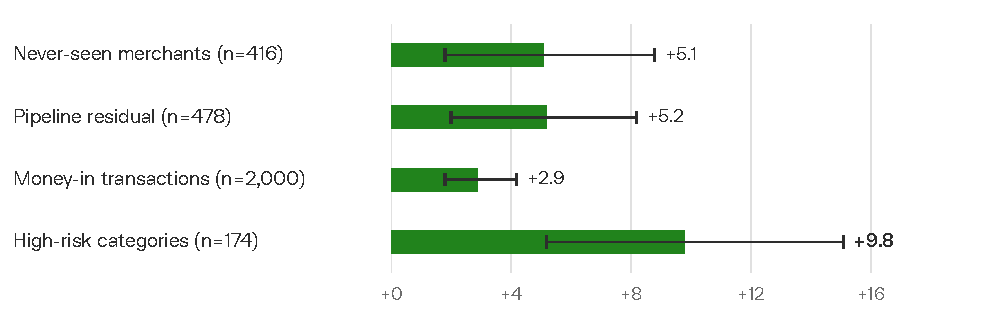
\includegraphics[width=\linewidth]{charts/fig-transformer.pdf}
\caption*{Leaf-level accuracy, mean of three seeds, paired bootstrap on the same rows. Every interval sits above zero. General-level gains are larger still, at 7 to 13 points.}
\end{figure}
Every accuracy criterion set at the start now clears with confidence intervals excluding zero. The remaining cost is speed: the transformer scores at about a third of the linear model's rate, which is roughly 70 CPU-minutes for the full Plaid table and has been judged acceptable for now. Quantisation would recover a factor of two to three if it becomes a constraint.

It is worth being clear about what the transformer did and did not do. The full-pipeline number moved by one point, because 76\% of transactions never reach the classifier. Its value is concentrated where the rules cannot help: on merchants nobody has labelled, and on the high-risk categories that the credit model cares about most.


% Edit this section directly. Styling is in raylo-report.sty.
\section{The credit-risk model and the new champion}
Categorisation is a means to an end: better features for the credit-risk model. The pipeline was run over every transaction for the 49,000 proposals with repayment outcomes, features were rebuilt from the resulting categories, and models were trained on the past and scored on a later window no model had seen. Both out-of-time windows are entirely Plaid, the live provider.

GINI measures how well a score rank-orders bad payers from good, where 0 is random and 1 is perfect. In credit-scoring terms the gaps below are large.

\subsection{From the August model to the champion}
The August report quoted a model capped at 50 features: GINI 0.477 on the three-month outcome and 0.564 on the six-month outcome, against a live model at 0.403 and 0.386. Two things have changed since.

The comparison was tightened. The live model is now refit on the full training window exactly as our models are, which brings its fair figure to 0.382 and 0.385. The as-of filter described in section 6 was applied. The capped model's numbers barely moved, to 0.477 and 0.562.

Then a stricter search was run for a stronger recipe. Where the 50-feature model used 40 individually tracked leaves and rolled the rest up, the champion search gave the model every observed leaf directly. For each of the 275 leaves it built five raw measures per applicant: the number of distinct months the leaf appears in, the transaction count, the debit count, and the debit and credit amounts. That is 1,654 columns once empty ones are dropped, on top of the 304 features already in use. A richer view normalised each by the applicant's totals (share of months, share of transactions, share of spend), reaching 3,150 columns. Eight recipes across XGBoost and LightGBM were compared, varying depth, regularisation, class weighting, a half-weight on Equifax rows and a recency decay that favours recent proposals.

Selection used three rolling validation windows that all sit before the published out-of-time window, and touched that window once, after the recipe was chosen. The final model is a blend of the two tree libraries, averaged over three seeds, with a calibration step so that its probabilities can be read as probabilities.


Out of time, the champion scores 0.533 on the three-month outcome and 0.618 on the six-month one: +0.056 [+0.030, +0.081] and +0.054 [+0.025, +0.084] over the 50-feature model, and +0.138 [+0.097, +0.179] and +0.200 [+0.158, +0.245] over the live model.
This is consistent with section 3: given every column, the taxonomy's detail is worth something to the six-month model, and per-leaf shares and averages are the form in which it is worth most. Persistence remains the dominant feature form (how many distinct months a category appears in matters more than how much was spent), and debt-structure features built from the priority-debt flag remain among the strongest.

\subsection{Holding the champion to 50 features}
The uncapped champion uses between 1,654 and 3,150 input columns, of which 700 to 1,450 carry weight in the fitted trees. That is a different governance proposition from a 50-feature model, where every column can be named, monitored for drift and explained to a reviewer. So the champion recipe was re-run under hard caps of 50, 100 and 200 features, ranking features by their average contribution across both tree libraries and all three seeds on the training window only. Nothing else was re-tuned.

The blend was re-examined at each cap. On the capped folds a single XGBoost matched or beat it on both outcomes, and LightGBM alone fell away at 50 features (0.559 on the six-month outcome). The blend was therefore dropped; the carried-forward model is a single XGBoost, which also keeps the learner identical to the live model's.


\Needspace{200pt}
{\small
\setlength{\TableWidth}{\dimexpr\linewidth-10\tabcolsep\relax}
\begin{longtable}{>{\raggedright\arraybackslash}p{0.34\TableWidth}>{\raggedright\arraybackslash}p{0.1\TableWidth}>{\raggedright\arraybackslash}p{0.15\TableWidth}>{\raggedright\arraybackslash}p{0.15\TableWidth}>{\raggedright\arraybackslash}p{0.26\TableWidth}}
\rowcolor{BlueTint}
\bfseries Champion recipe, scored out of time & \bfseries Features & \bfseries 3-month & \bfseries 6-month & \bfseries 6-month gap to uncapped, 95\% CI \\ \midrule
\endfirsthead
\rowcolor{BlueTint}
\bfseries Champion recipe, scored out of time & \bfseries Features & \bfseries 3-month & \bfseries 6-month & \bfseries 6-month gap to uncapped, 95\% CI \\ \midrule
\endhead
Live model, fair refit &  & 0.382 & 0.385 &  \\ \addlinespace[4pt]
August model, single XGBoost & 50 & 0.477 & 0.562 &  \\ \addlinespace[4pt]
\rowcolor{PeachTint}
Champion recipe, single XGBoost, carried forward & 50 & 0.508 & 0.588 & -0.030 [-0.052, -0.009] \\ \addlinespace[4pt]
Champion recipe, XGBoost + LightGBM blend & 50 & 0.508 & 0.583 & -0.035 [-0.057, -0.014] \\ \addlinespace[4pt]
Champion recipe, blend & 100 & 0.520 & 0.589 & -0.029 [-0.047, -0.010] \\ \addlinespace[4pt]
Champion recipe, blend & 200 & 0.529 & 0.600 & -0.018 [-0.032, -0.004] \\ \addlinespace[4pt]
Champion, uncapped & 1,654 to 3,150 & 0.533 & 0.618 &  \\ \addlinespace[4pt]
\bottomrule
\end{longtable}}
\begin{figure}[H]
\centering
\ChartTitle{Figure 8. Out-of-time GINI: live model, August taxonomy model, and the champion at each feature cap}
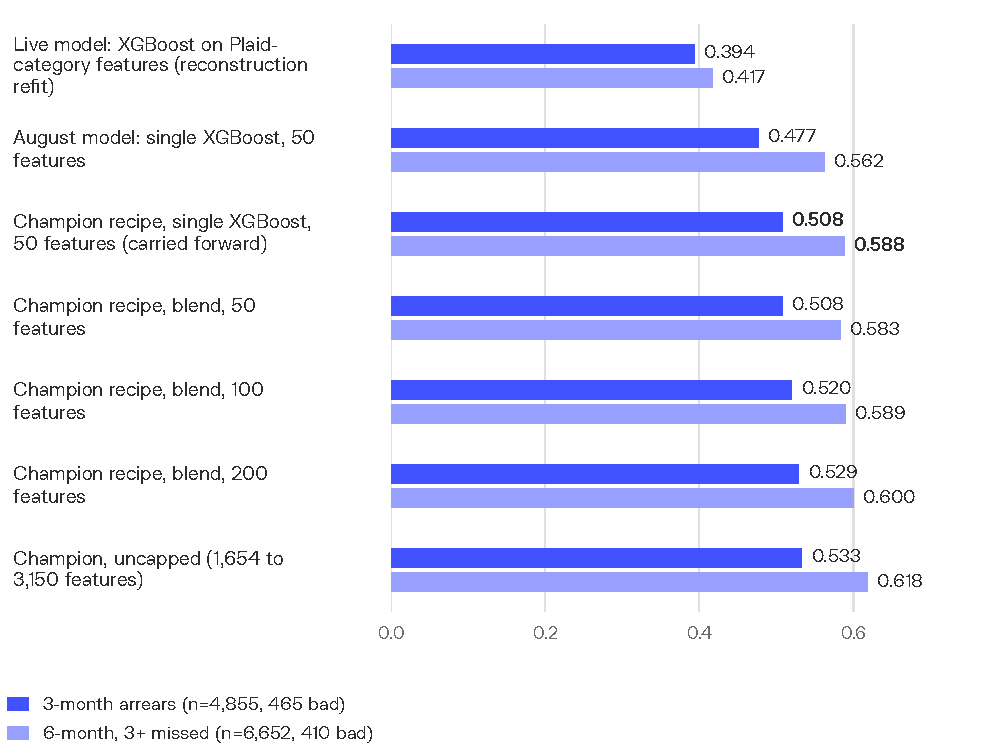
\includegraphics[width=\linewidth]{charts/fig-gini.pdf}
\caption*{Both windows are entirely Plaid. From the 50-feature rows upward the recipe is identical; only the number of columns and the use of a second tree library change.}
\end{figure}
The cap has a real cost and no convenient knee: on the six-month outcome the model is still improving at 200 features. Roughly a third of the champion's gain over the August model is the recipe, which survives a cap, and two thirds is the width, which does not. At 50 features the single-XGBoost recipe beats the August model by +0.031 on the three-month outcome (interval excluding zero) and by +0.024 on the six-month one (interval touching zero).

The 50-feature single-XGBoost champion is carried forward as the reference for the prospective test and for anything that approaches production. Its uplift over the live model, 0.13 GINI on the three-month outcome and 0.20 on the six-month, is what a lending decision would act on, and that barely changes with the cap. The cap gives up the last two to four points in exchange for a model whose every input can be named. The uncapped champion is kept as the ceiling reference; the table above shows what each step of width would buy back.

\begin{tcolorbox}[colback=BlueTint,colframe=Blue,boxrule=0pt,leftrule=2pt,arc=3mm]
Both champions are development recipes. Their out-of-time windows had been used in earlier experiment work, so 0.588 and 0.618 should be read as upper estimates until the prospective test in section 13 is run on a window nobody has touched.
\end{tcolorbox}

% Edit this section directly. Styling is in raylo-report.sty.
\section{Adding text to the risk model}
A separate programme, run in its own repository over the first week of September, asked a different question. The champion sees each applicant as a table of category counts. Could a model that reads the applicant's raw transaction sequence, in order, with the bank's own wording, find signal that the counts lose? This is the thesis behind several published ``transaction foundation model'' efforts, and it was tested here in two stages.

\subsection{How the two learned scores work}
Both approaches in this section end the same way: as a single number per applicant that is handed to the tree model as one more column. They differ in what they read.

\textbf{The text encoder} is the same kind of encoder transformer described in section 9, but used without any fine-tuning. An off-the-shelf model (bge-base, trained by its authors on general English) reads each bank narrative and produces a 768-number summary. Those summaries are averaged across all of an applicant's transactions, so the result is one vector describing the flavour of their statement as a whole, without any category having been assigned. A small logistic model, fitted on our own outcome data, turns that vector into one risk score. Nothing in this path knows about our taxonomy; it captures whatever the wording of the transactions says that the categories do not.

\textbf{The sequence transformer} reads the applicant, not the narrative. Each transaction becomes one event carrying its amount band, its timing relative to the application, its direction, the taxonomy leaf our categoriser gave it, and a compressed text vector. The events are laid out in date order, up to 1,024 of them, and a transformer reads the whole sequence at once, so a payday loan the day after a gambling spree can be understood as a pattern rather than two separate counts. It was pretrained on 48,000 applicants' histories with the sequence version of fill-in-the-blank, hiding one event and asking the model to reconstruct it, and then a small head was trained on repayment outcomes. Its output is again one number per applicant.

\begin{figure}[H]
\centering
\ChartTitle{Figure 8a. How the two learned scores are produced for one applicant}
\resizebox{\linewidth}{!}{%
\begin{tikzpicture}[
  x=1mm,y=1mm,font=\footnotesize,
  box/.style={draw=Blue,fill=BlueTint,rounded corners=1.2mm,line width=0.4pt,align=center,inner sep=2mm,text width=34mm},
  boxp/.style={draw=Peach,fill=PeachTint,rounded corners=1.2mm,line width=0.4pt,align=center,inner sep=2mm,text width=34mm},
  data/.style={draw=Muted,fill=white,rounded corners=1.2mm,line width=0.4pt,align=left,inner sep=2mm,text width=40mm},
  result/.style={draw=Blue,fill=Blue,text=white,rounded corners=1.2mm,line width=0.4pt,align=center,inner sep=2mm,text width=34mm},
  lab/.style={font=\scriptsize\color{Muted},align=left},
  arr/.style={-{Stealth[length=2mm]},line width=0.5pt,color=Muted}]
  \node[data,text width=44mm] (app) at (0,-8) {\textbf{One applicant, 90 days}\\about 300 transactions, each with date, amount, direction, narrative and our category};
  % text path
  \node[lab,anchor=west] at (54,22) {\textbf{Text score} (locked)};
  \node[box] (enc) at (74,8) {\textbf{Text encoder}\\bge-base reads each narrative\\$\rightarrow$ 300 vectors of 768 numbers};
  \node[box] (mean) at (118,8) {\textbf{Average}\\one vector for the whole statement};
  \node[result] (probe) at (162,8) {\textbf{Probe}\\logistic fit on outcomes\\$\rightarrow$ one score};
  % sequence path
  \node[lab,anchor=west] at (54,-14) {\textbf{Sequence-encoder score} (challenger)};
  \node[boxp] (ev) at (74,-28) {\textbf{Events in date order}\\amount band, timing, direction, taxonomy leaf, text vector};
  \node[boxp] (seq) at (118,-28) {\textbf{Sequence transformer}\\15M parameters, frozen; attends across all events};
  \node[result] (head) at (162,-28) {\textbf{Attention head}\\trained on outcomes\\$\rightarrow$ one score};
  % xgb
  \node[data,text width=40mm] (xgb) at (212,-10) {\textbf{Risk model}\\single XGBoost on 50 taxonomy features + text score (+ encoder score in the challenger recipe)\\$\rightarrow$ probability of default};
  \node[lab,anchor=north,align=center] (feat) at (212,-30) {the 50 taxonomy features come\\from the categorised transactions\\(section 10)};
  \draw[arr] (app.east) -- ++(4,0) |- (enc.west);
  \draw[arr] (app.east) -- ++(4,0) |- (ev.west);
  \draw[arr] (enc) -- (mean); \draw[arr] (mean) -- (probe);
  \draw[arr] (ev) -- (seq); \draw[arr] (seq) -- (head);
  \draw[arr] (probe.east) -- ++(3,0) |- ([yshift=4mm]xgb.west);
  \draw[arr,dashed] (head.east) -- ++(3,0) |- ([yshift=-4mm]xgb.west);
  \draw[arr] (feat.north) -- (xgb.south);
\end{tikzpicture}}
\caption*{Both paths reduce an applicant's transactions to one number that the tree model treats like any other feature. The text path runs one frozen encoder; the sequence path needs the categoriser's leaf, a second text encoder for its inputs, and the sequence model itself, which is why it is the challenger rather than the primary recipe.}
\end{figure}

What this means for the risk model: the trees already see how much, how often and in how many months each category appears. The text score adds what the words say beyond the category, for instance that an ``unclassified transfer'' narrative reads like a loan repayment. The sequence score adds order and timing, which counts lose. Neither replaces the trees; each supplies one column the trees could not compute for themselves, and the results below show how much each column is worth.

\subsection{Stage one: do text embeddings carry credit signal at all}
The cheapest test first. Each distinct bank narrative (2.9 million strings) was turned into a vector by a frozen off-the-shelf sentence encoder, the vectors were averaged per applicant, and a logistic regression was fitted on the average. With no categories and no hand-built features, that probe matched the production-spec GBM refit on the same population. The text does carry signal. Compressed to 32 columns and added to the taxonomy model, it gave a small and unstable lift.

\subsection{Stage two: a sequence transformer over transactions}
A transformer was then built to read up to 1,024 transactions per applicant, each represented by its amount bucket, timing, direction and text vector. It was pretrained with a masked-event objective, the sequence equivalent of fill-in-the-blank, on 48,000 applicants' histories, and read out first with a linear probe and later with fine-tuning. The versions are worth listing because each was built to test one thing.


{\small
\setlength{\TableWidth}{\dimexpr\linewidth-8\tabcolsep\relax}
\begin{longtable}{>{\raggedright\arraybackslash}p{0.16\TableWidth}>{\raggedright\arraybackslash}p{0.36\TableWidth}>{\raggedright\arraybackslash}p{0.33\TableWidth}>{\raggedright\arraybackslash}p{0.15\TableWidth}}
\rowcolor{BlueTint}
\bfseries Version & \bfseries What changed & \bfseries Why & \bfseries GINI, six-month \\ \midrule
\endfirsthead
\rowcolor{BlueTint}
\bfseries Version & \bfseries What changed & \bfseries Why & \bfseries GINI, six-month \\ \midrule
\endhead
v1 & 5 million parameters, raw fields only, 26 laptop-minutes & Establish a floor & 0.450 \\ \addlinespace[4pt]
v2, v3 & Longer training; 56\% more data including unlabelled recent applicants & Rule out data and training length as the limit & 0.473 \\ \addlinespace[4pt]
v4 & Each transaction also carries our taxonomy leaf as an input token & Test whether the model needs categories or can derive them & 0.546 \\ \addlinespace[4pt]
v5 & Leaf token made provider-blind (general category where the leaf came from a provider crosswalk) & The raw leaf let the model identify the provider perfectly, which would not transfer & 0.561 \\ \addlinespace[4pt]
v5 fine-tuned & Full fine-tuning with attention pooling & Test whether the readout, not the representation, was the limit & 0.551 \\ \addlinespace[4pt]
v6 & Three times the parameters (15 million) & Test capacity & 0.576 to 0.586 \\ \addlinespace[4pt]
\rowcolor{PeachTint}
Champion, refit on the same population &  &  & 0.616 \\ \addlinespace[4pt]
\bottomrule
\end{longtable}}
\begin{figure}[H]
\centering
\ChartTitle{Figure 9. Sequence transformer versions against the champion, six-month GINI on 6,252 applicants}
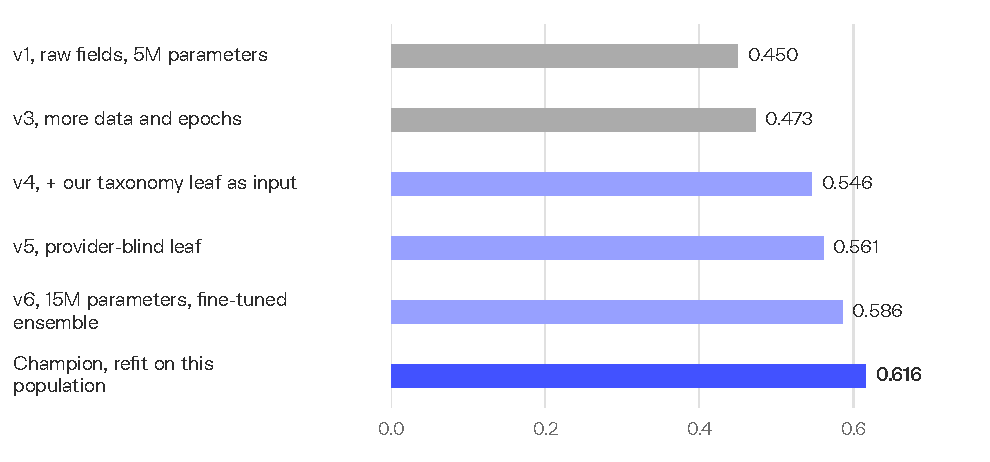
\includegraphics[width=\linewidth]{charts/fig-seq.pdf}
\caption*{The step from v3 to v4 is the category token. Everything after it is inside the noise of 397 bad outcomes. Stacked on the champion, no version added a significant gain.}
\end{figure}
The pattern is clear in hindsight. Without categories the sequence model plateaued at about 0.47 regardless of data or epochs. Given our leaf as an input, it jumped to the level of the 50-feature taxonomy XGBoost. Every further lever, fine-tuning, attention pooling and tripling the size, moved it a little, and the best configuration is statistically level with the champion but below it on both metrics. The bigger model overfitted within two epochs because there are only 2,200 bad outcomes to learn from; label scarcity, not model capacity, capped every configuration.

The sequence-model results in this section were measured against the uncapped champion, refit on that repository's population (GINI 0.616). The text-score stacking was then re-run against the 50-feature capped champion once it became the reference; those results are at the end of the section.

Stacked on the uncapped champion as an extra feature, the sequence model added nothing significant. The champion's thousands of leaf-level columns already contain what the sequence model had learned from categories, and at that point it was parked. The picture changed once the 50-feature capped champion became the reference, as the last part of this section shows.

\subsection{What did add value: one text score}
What remains in the raw text after the categories are accounted for is small but real, and the simplest extraction captures it. A frozen sentence encoder embeds each description, the vectors are averaged per applicant, and a small logistic model turns the average into one risk score, added to the champion as a single column. That single number beat 32 compressed columns, and it is far easier to monitor.

Eight encoders were compared in that role, from 22 million to 568 million parameters, including our own domain-pretrained DistilBERT from section 9. All landed in one narrow band of roughly +0.01 PR-AUC on the champion. Encoder size and family do not matter here, which is itself informative: the lift is a property of the residual free text, not of the encoder. bge-base was chosen because both of its deltas exclude zero and it runs on a laptop CPU. Our own encoder was fractionally ahead on the point estimate and half the cost to run, but not distinguishably better, and it had seen the test period's text during unsupervised pretraining, so it is recorded as the preferred replacement candidate pending the prospective test.

\begin{figure}[H]
\centering
\ChartTitle{Figure 10. PR-AUC lift from one text score, on the uncapped and the 50-feature champion (95\% CIs)}
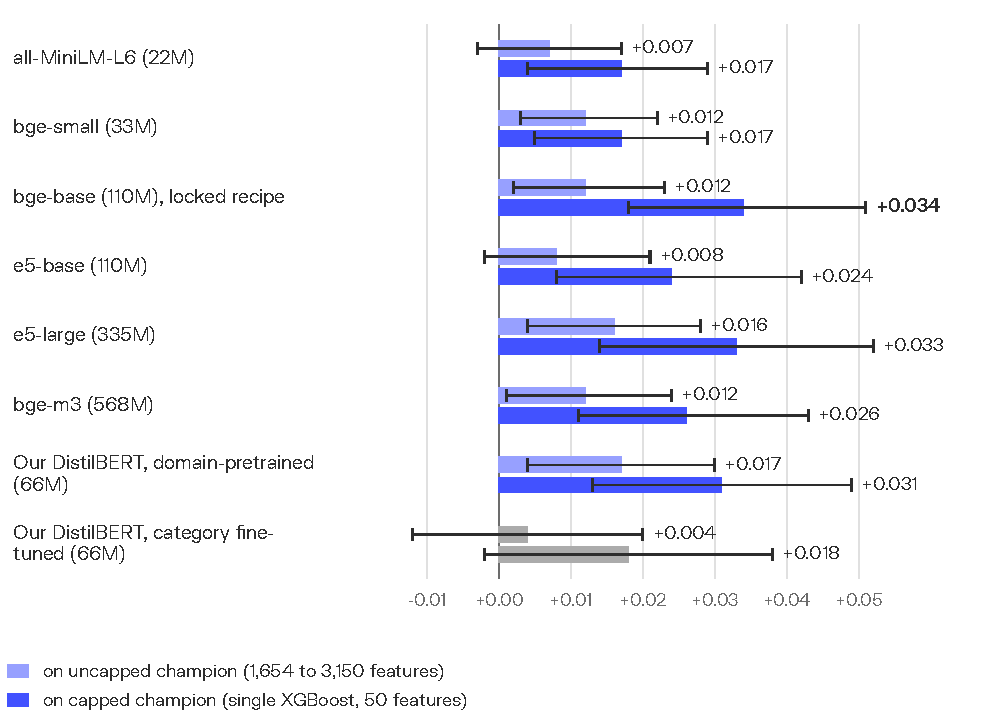
\includegraphics[width=\linewidth]{charts/fig-stack.pdf}
\caption*{On the uncapped champion, eight encoders spanning a 25-fold range in size land in one band: the lift is a property of the free text the taxonomy misses, not of the encoder. On the 50-feature single-XGBoost champion the same scores are worth two to three times as much and every GINI interval excludes zero, with the ordering unchanged: bge-base, e5-large and our domain-pretrained encoder share the top, the 568M encoder buys nothing over them, and the category-fine-tuned encoder is weakest.}
\end{figure}

{\small
\setlength{\TableWidth}{\dimexpr\linewidth-6\tabcolsep\relax}
\begin{longtable}{>{\raggedright\arraybackslash}p{0.4\TableWidth}>{\raggedright\arraybackslash}p{0.28\TableWidth}>{\raggedright\arraybackslash}p{0.32\TableWidth}}
\rowcolor{BlueTint}
\bfseries Six-month outcome, 6,252 applicants, 397 bad & \bfseries PR-AUC & \bfseries GINI \\ \midrule
\endfirsthead
\rowcolor{BlueTint}
\bfseries Six-month outcome, 6,252 applicants, 397 bad & \bfseries PR-AUC & \bfseries GINI \\ \midrule
\endhead
Champion alone & 0.290 & 0.616 \\ \addlinespace[4pt]
\rowcolor{PeachTint}
Champion + bge-base text score (locked recipe) & 0.302 (+0.012 [+0.002, +0.023]) & 0.625 (+0.009 [+0.001, +0.018]) \\ \addlinespace[4pt]
Champion + our domain-pretrained encoder score & 0.307 (+0.017 [+0.004, +0.030]) & 0.626 (+0.010 [+0.000, +0.019]) \\ \addlinespace[4pt]
Champion + sequence transformer score & not significant & not significant \\ \addlinespace[4pt]
\bottomrule
\end{longtable}}
\subsection{Both scores on the capped champion}
The figures in this subsection are measured against the single-XGBoost 50-feature champion adopted in section 10, refit on that repository's population. A smaller base model leaves more for a learned score to explain, and that is what the re-run against the capped champion shows. Two scores were tested, each one column. The text score is the bge-base recipe above. The encoder score is the sequence transformer in its lightest deployable form: the 15-million-parameter pretrained encoder kept frozen, with only a small attention-pooling head trained on outcomes, so one model and one head would run in production rather than the five-fold ensemble used to produce honest training scores.


{\small
\setlength{\TableWidth}{\dimexpr\linewidth-10\tabcolsep\relax}
\begin{longtable}{>{\raggedright\arraybackslash}p{0.32\TableWidth}>{\raggedright\arraybackslash}p{0.1\TableWidth}>{\raggedright\arraybackslash}p{0.1\TableWidth}>{\raggedright\arraybackslash}p{0.24\TableWidth}>{\raggedright\arraybackslash}p{0.24\TableWidth}}
\rowcolor{BlueTint}
\bfseries Six-month outcome, 6,252 applicants, 397 bad & \bfseries PR-AUC & \bfseries GINI & \bfseries \ensuremath{\Delta}PR-AUC [95\% CI] & \bfseries \ensuremath{\Delta}GINI [95\% CI] \\ \midrule
\endfirsthead
\rowcolor{BlueTint}
\bfseries Six-month outcome, 6,252 applicants, 397 bad & \bfseries PR-AUC & \bfseries GINI & \bfseries \ensuremath{\Delta}PR-AUC [95\% CI] & \bfseries \ensuremath{\Delta}GINI [95\% CI] \\ \midrule
\endhead
Capped champion, single XGBoost, 50 features, refit & 0.265 & 0.588 &  &  \\ \addlinespace[4pt]
Sequence transformer alone, single frozen model & 0.250 & 0.576 & not significant & not significant \\ \addlinespace[4pt]
Capped champion + text score (locked recipe, 51 columns) & 0.299 & 0.611 & +0.034 [+0.018, +0.051] & +0.024 [+0.012, +0.035] \\ \addlinespace[4pt]
Capped champion + encoder score & 0.296 & 0.617 & +0.031 [+0.011, +0.051] & +0.029 [+0.016, +0.043] \\ \addlinespace[4pt]
\rowcolor{PeachTint}
Capped champion + text score + encoder score (52 columns) & 0.322 & 0.629 & +0.056 [+0.033, +0.080] & +0.042 [+0.025, +0.058] \\ \addlinespace[4pt]
Uncapped champion, refit, for reference & 0.290 & 0.616 &  &  \\ \addlinespace[4pt]
\bottomrule
\end{longtable}}
Three things follow. The text score is worth about three times what it was on the uncapped champion (+0.024 GINI against +0.009), because the smaller base leaves the free text unexplained. The sequence model, which added nothing on the uncapped champion, adds a clear +0.029 GINI on the capped one for the same reason: its value was always category dynamics at the leaf level, which 3,150 columns held directly and 50 do not. And the two scores are additive. Fifty engineered features plus two learned columns reach 0.322 / 0.629, above the uncapped champion on both metrics, with each column nameable and monitorable.

The cost is in the serving path rather than the feature count. The text score needs one text encoder over every description. The encoder score needs a second text encoder for its inputs, the sequence model itself, and our categoriser's leaf on every transaction. That is why the text-only recipe stays locked as the primary and the two-score version goes to the prospective test as the challenger: both have now been evaluated many times against the same 397 bad outcomes, and a cohort nobody has touched is the only clean arbiter left. Substituting our own domain-pretrained encoder for bge-base in the text score gives near-identical results (0.296 / 0.613 against 0.299 / 0.611) at about half the serving cost and with no third-party model in the decision path. The decision taken is to keep bge-base as the locked encoder and to register ours as the named alternative for the prospective test. The reason is evidential rather than technical: our encoder's pretraining corpus included the test period's transactions (no labels, vocabulary exposure only), while bge-base has none, so the cleaner comparison is the one to carry until a cohort nobody has touched can score both once. If ours holds level there, the cost and ownership case decides it.

{\small\color{Muted} PR-AUC is the area under the precision-recall curve, a second ranking metric that weights the rare bad outcomes more heavily than GINI does. Both are reported because on a few hundred bad outcomes they can move independently.\par}

% Edit this section directly. Styling is in raylo-report.sty.
\section{Why these architectures and not others}
Two different problems sit in this work and they want different tools: reading text (a merchant string and narrative into one of 275 categories) and ranking applicants (a table of per-applicant numbers into a default probability). Each choice was tested against the simpler alternative before being kept.

\subsection{For reading text}

{\small
\setlength{\TableWidth}{\dimexpr\linewidth-6\tabcolsep\relax}
\begin{longtable}{>{\raggedright\arraybackslash}p{0.29\TableWidth}>{\raggedright\arraybackslash}p{0.26\TableWidth}>{\raggedright\arraybackslash}p{0.45\TableWidth}}
\rowcolor{BlueTint}
\bfseries Approach & \bfseries Why it was tested & \bfseries Outcome \\ \midrule
\endfirsthead
\rowcolor{BlueTint}
\bfseries Approach & \bfseries Why it was tested & \bfseries Outcome \\ \midrule
\endhead
Dictionary and rules & Deterministic, explainable, free at runtime, and the only way to encode facts one row cannot reveal. & Resolve 58\% of live rows at about 90\% accuracy. Live. \\ \addlinespace[4pt]
Character TF-IDF + linear SVM & The standard baseline for short noisy text. Anything fancier must beat it. & Serving since August; v8 is the reference. Logistic regression and an exact SVM solver both lost to it. \\ \addlinespace[4pt]
Frontier language models & Set the ceiling and produce labels. Gemini reads unseen merchants at 84\%. & Used offline as a two-model committee. Too slow, costly and unauditable per transaction. \\ \addlinespace[4pt]
Fine-tuned small generative models & Could a small generative model match the frontier and be served locally? & 50 to 54\% on unseen merchants. Rejected. \\ \addlinespace[4pt]
Generic sentence encoder + classifier & Cheapest neural option; tests whether general English transfers. & Loses to the SVM, badly on risk categories. Rejected. \\ \addlinespace[4pt]
Domain-pretrained encoder transformer & Encoder because the output is a closed choice; domain pretraining because the literature and our own failures both said that is where the gain is. & +5 points on novel merchants, +10 on risk categories over the SVM. Candidate for the ML tier. \\ \addlinespace[4pt]
Off-the-shelf rules engine & Could a purpose-built product host the tiers? & Reproduces the dictionary and nothing else; two tiers inexpressible. Rejected. \\ \addlinespace[4pt]
\bottomrule
\end{longtable}}
\textbf{Why not a larger encoder still?} Moving from 29 to 66 million parameters bought four points on the risk set; that was the scale lever. Larger models cost throughput, already a third of the SVM's, and the encoder sweep in section 11 showed that size stops mattering once the domain is covered. If the classifier needs another step, more consensus labels are cheaper than more parameters.

\textbf{Why not use the language model at decision time?} Cost and latency per transaction, non-deterministic outputs (identical calls disagreed on 12\% of rows), no audit trail beyond the model's say-so, and a vendor dependency inside a credit decision.

\subsection{For ranking applicants}

{\small
\setlength{\TableWidth}{\dimexpr\linewidth-6\tabcolsep\relax}
\begin{longtable}{>{\raggedright\arraybackslash}p{0.29\TableWidth}>{\raggedright\arraybackslash}p{0.26\TableWidth}>{\raggedright\arraybackslash}p{0.45\TableWidth}}
\rowcolor{BlueTint}
\bfseries Approach & \bfseries Why it was tested & \bfseries Outcome \\ \midrule
\endfirsthead
\rowcolor{BlueTint}
\bfseries Approach & \bfseries Why it was tested & \bfseries Outcome \\ \midrule
\endhead
Logistic regression & The classic scorecard form; shows how much signal the categories carry alone. & 0.33 GINI. Useful for reading feature strength; not the production learner. \\ \addlinespace[4pt]
XGBoost on 50 taxonomy features & The live model is an XGBoost, so this isolates the value of our categories with the learner held constant. & 0.56 against 0.42 live. The August headline. \\ \addlinespace[4pt]
XGBoost + LightGBM blend on leaf-level features & Does giving the trees every leaf beat 50 aggregated features? & 0.62 uncapped as a blend; 0.59 held to 50 features as a single XGBoost, which matched the blend at every cap. The capped single model is carried forward, pending the prospective test. \\ \addlinespace[4pt]
Sequence transformer over transactions & The foundation-model thesis: order and timing may carry signal the counts lose. & Level with the taxonomy XGBoost once given our categories; nothing on top of the uncapped champion; +0.029 GINI as one column on the 50-feature champion. Challenger for the prospective test. \\ \addlinespace[4pt]
Frozen text embedding as one score & One calibrated, monitorable number is a better feature than 32 opaque columns. & +0.034 PR-AUC and +0.024 GINI on the 50-feature champion, both CIs excluding zero. Locked recipe. \\ \addlinespace[4pt]
\bottomrule
\end{longtable}}
\textbf{Why gradient-boosted trees and not a neural network?} On tabular data with a few thousand bad outcomes, boosted trees remain the strongest and most explainable learner, and the live model is one, so the comparison is clean. The neural option was tested properly, as a sequence model, and did not beat the trees once both saw the same categories. Where it does earn a place is as one learned column feeding the trees, not as their replacement.


\clearpage
% Edit this section directly. Styling is in raylo-report.sty.
\section{Status, caveats and next steps}
\subsection{Where things stand}
The taxonomy, pipeline, dictionary and evaluation methodology are complete. Classifier v8 and the transformer are both measured against merchant-disjoint evaluation sets, and the transformer clears every accuracy criterion. The 50-feature single-XGBoost champion is the reference credit model, with the uncapped champion as the ceiling. The text-score recipe is locked (+0.024 GINI on the capped model) and the two-score version (0.629) is the registered challenger. Nothing is yet referenced by a production model or scheduled job.

\subsection{Caveats to carry into any decision}
\begin{itemize}
\item The champion's 0.588 (capped, single XGBoost) and 0.618 (uncapped blend) are development numbers. Their test windows were used in earlier work, and the like-for-like uplift over the live model is the whole bundle of taxonomy, features and learner; a same-feature-count ablation was inconclusive.
\item Each out-of-time window rests on a few hundred bad outcomes. The gaps to the live model are far larger than that noise; the text-score and encoder-score lifts are not, and both recipes have been evaluated repeatedly against this one window. The prospective cohort is the only clean arbiter left.
\item The 400-row risk evaluation set is unseen rows of a known population, not an unseen population. Two risk leaves (debt collection, casino) remain thin.
\item Half of all transactions resolve through provider-derived tiers, so no feature built from categories is fully provider-blind. Transfer from Equifax history to Plaid traffic is verified empirically rather than assumed.
\end{itemize}
\subsection{Next steps, in order}
\begin{enumerate}
\item \textbf{Promote the machine-learning tier.} Classifier v8 now, as a zero-risk step; the transformer once a serving artefact exists. Either needs a scheduled per-row categorisation job keyed by transaction id.
\item \textbf{Score the locked confirmation set once,} at go/no-go, and never again.
\item \textbf{Run the prospective test.} Freeze taxonomy, dictionary, classifier, feature SQL and the champion recipe with an effective date, then score the next matured cohort (February to April 2026 outcomes, mature by about November) once against pre-agreed bars. Two recipes are registered, the capped champion plus text score as primary and plus both learned scores as challenger, each scored with bge-base and with our own encoder. This is the gate for the champion, both scores and the encoder swap.
\item \textbf{Close the remaining data gaps:} thin risk leaves, and a human blind slice on the risk tranche.
\item \textbf{Fix the 90-day history request.} Every Plaid Asset Report since go-live asks for exactly 90 days. That is a Raylo-side parameter, not a Plaid limit, and it caps every history-based feature. Probably the cheapest uplift available, and it belongs to whoever owns the Plaid integration.
\end{enumerate}
{\small\color{Muted} Evidence base: dated experiment reports in the repository's data directory, the programme review of 2 September, the programme summary of 5 September, and the OB-transformer repository's phase-one and phase-two write-ups.\par}

\end{document}
